\documentclass[conference]{IEEEtran}
%\usepackage{spconf,amsmath,amssymb,graphicx}
\usepackage{amsmath,amssymb,graphicx}

% Example definitions.
% --------------------
% nice symbols for real and complex numbers
\newcommand{\R}[0]{\mathbb{R}}
\newcommand{\C}[0]{\mathbb{C}}
% bold paragraph titles
\newcommand{\mypar}[1]{{\bf #1.}}

\begin{document}

\title{A Stencil computation optimization}


\author{\IEEEauthorblockN{Ivan Buccella}
\IEEEauthorblockA{Department of Computer Science\\
 University of Salerno\\
 Italy}
}

\maketitle

\begin{abstract}
Describe in concise words what you do, why you do it (not necessarily
in this order), and the main result.  The abstract has to be
self-contained and readable for a person in the general area. You
should write the abstract last.
\end{abstract}

\section{Introduction}\label{sec:intro}

Stencil computation has been a research topics for decades in a variety of domains including computational electromagnetics \cite{taflove}, solution of PDEs using finite difference or finite volume discretizations \cite{smith}, and image processing for CT and MRI imaging \cite{cong-huang-zou}\cite{cong-zou}. In the finite difference computation process, stencil computation is often iteratively used to solve the differential operator. In these scientific and engineering applications, Stencil is often the most vital and time-consuming computing kernel.\cite{su-zhang-mei}

The general computation pattern of stencil computation is that the central point accumulates the contributions of neighbor points in every axis of the Cartesian coordinate system.\cite{su-zhang-mei} The number of neighbor points in each axis or grid step of the stencil computation corresponds to the accuracy of the stencil. The more neighbor elements involved in the computation, the higher accuracy the computation obtains. The computation is then repeated for every point of the grid domain as an iterative operator of the PDEs. Due to the structure of the stencil computation two inherent problems exist:
\begin{itemize}
	\item First, it is the non-continuous memory access pattern. There exist distances among elements needed for the computation except those in the innermost or unit-stride dimension. Many more cycles in latencies are required to access these points. 
	\item Second, it is the low arithmetic intensity and poor data reuse. Just one point is updated with all the elements loaded. The data reuse between two updates is also limited within the unit-stride dimension, while the other dimensions' elements that are expensive to access have no data reuse at all.
\end{itemize}


\mypar{Motivation} 
On the stencil computation various optimization approaches have been discussed. The main contributions for stencil optimization can be divided into two aspects: blocking and parallelism optimizations.\cite{su-zhang-mei}

Blocking optimizations aim at improving the data locality of both space and time dimensions. They are highly related to the tiling strategies widely employed in the modern multi-level cache hierarchy architectures.
 
Parallelism optimizations refer to the techniques that explore parallelism at diverse levels, including data-level parallelism, such as SIMD, thread-level parallelism, such as block decomposition, and instruction-level parallelism. They tend to make full use of the potential advantages of modern processors' many- or multi-core architectures. 

However, these optimizations can be categorized according to their complexity of implementation (programmer efforts), benefit improvement (performance) and implementation tightness regarding hardware (dependence) \cite{cruz}.

\mypar{Related work} 
In the article `\textit{Acceleration of real-life stencil codes on GPUs}' \cite{barigou} there is a detailed description of what the loop tiling transformation, the CUDA programming model and GPU architecture consists. Then, it explores the possible tiling approaches that can be applied on such stencil patterns; it describes 3 interesting approaches: 2D tiles, time-skewing+time-tiling transformation and performing redundant computations inside tiles.

In the article `\textit{High-Performance Code Generation for Stencil Computations on GPU Architectures}' \cite{holewinski-pouchet-sadayappan} 
is introduced an automatic code generation scheme for stencil computations on GPU architectures. This scheme uses overlapped tiling to provide efficient time tiling on GPU architectures, which are massively threaded but are susceptible to performance degradation due to branch divergence and a lack of memory coalescing. 

However, what we will try to do is to apply multi-core architecture optimizations using OpenMP, instead of CUDA programming models and GPU architecture.

\section{Background}\label{sec:background}

In order to understand the described work it is important to know something about multi-core, and code optimizations using OpenMP.

\mypar{The Multi-Core architecture}
Multicore refers to an architecture in which a single physical processor incorporates the core logic of more than one processor. A single integrated circuit is used to package or hold these processors. These single integrated circuits are known as a die. Multicore architecture places multiple processor cores and bundles them as a single physical processor. The objective is to create a system that can complete more tasks at the same time, thereby gaining better overall system performance. \cite{techopedia}

\mypar{OpenMP}
The OpenMP API supports multi-platform shared-memory parallel programming in C/C++ and Fortran. The OpenMP API defines a portable, scalable model with a simple and flexible interface for developing parallel applications on platforms from the desktop to the supercomputer. \cite{openmp}

\mypar{Loop Interchange}
In compiler theory, loop interchange is the process of exchanging the order of two iteration variables used by a nested loop. The variable used in the inner loop switches to the outer loop, and vice versa. It is often done to ensure that the elements of a multi-dimensional array are accessed in the order in which they are present in memory, improving locality of reference. \cite{loop-interchange}

\mypar{Optimization Flags}
Without any optimization option, the compiler's goal is to reduce the cost of compilation and to make debugging produce the expected results. Statements are independent: if you stop the program with a breakpoint between statements, you can then assign a new value to any variable or change the program counter to any other statement in the function and get exactly the results you expect from the source code. 
Turning on optimization flags makes the compiler attempt to improve the performance and/or code size at the expense of compilation time and possibly the ability to debug the program. 
The compiler performs optimization based on the knowledge it has of the program. 
Depending on the target and how the compiler was configured, a slightly different set of optimizations may be enabled at each -O level (\textit{-O1},\textit{-O2},\textit{-O3},\textit{-O4}).\cite{optimization-flags}

\mypar{Parallel Loops}
A parallel for loop is a for loop in which the statements in the loop can be run in parallel: on separate cores, processors or threads. 
In OpenMp the \textit{parallel loop} construct is a shortcut for specifying a parallel construct containing a loop construct with one or more associated loops and no other statements. \cite{parallel-loops}

\mypar{Loop Tiling}
Loop tiling, also known as loop blocking, is a loop transformation that exploits spatial and temporal locality of data accesses in loop nests. This transformation allows data to be accessed in blocks (tiles), with the block size defined as a parameter of this transformation. Each loop is transformed in two loops: one iterating inside each block (intratile) and the other one iterating over the blocks (intertile). \cite{loop-tiling}

\section{Your Proposed Method}\label{sec:yourmethod}

Now comes the ``beef'' of the report, where you explain what you
did. Again, organize it in paragraphs with titles. As in every section
you start with a very brief overview of the section.

In this section, structure is very important so one can follow the technical content.

Mention and cite any external resources that you used including libraries or other code.

\section{Experimental Results}\label{sec:exp}

Here you evaluate your work using experiments. You start again with a
very short summary of the section. The typical structure follows.

\mypar{Experimental setup} Specify the platform (processor, frequency, maybe OS, maybe cache sizes)
as well as the compiler, version, and flags used. If your work is about performance, 
I strongly recommend that you play with optimization flags and consider also icc for additional potential speedup.

Then explain what kind of benchmarks you ran. The idea is to give enough information so the experiments are reproducible by somebody else on his or her code.
For sorting you would talk about the input sizes. For a tool that performs NUMA optimization, you would specify the programs you ran.

\mypar{Results}
Next divide the experiments into classes, one paragraph for each. In each class of experiments you typically pursue one questions that then is answered by a suitable plot or plots. For example, first you may want to investigate the performance behavior with changing input size, then how your code compares to external benchmarks.


{\bf Comments:}
\begin{itemize}
\item Create very readable, attractive plots (do 1 column, not 2 column plots
for this report) with readable font size. However, the font size should also not be too large; typically it is smaller than the text font size.
An example is in Fig.~\ref{fftperf} (of course you can have a different style).
\item Every plot answers a question. You state this question and extract the
answer from the plot in its discussion.
\item Every plot should be referenced and discussed.
\end{itemize}

\begin{figure}\centering
  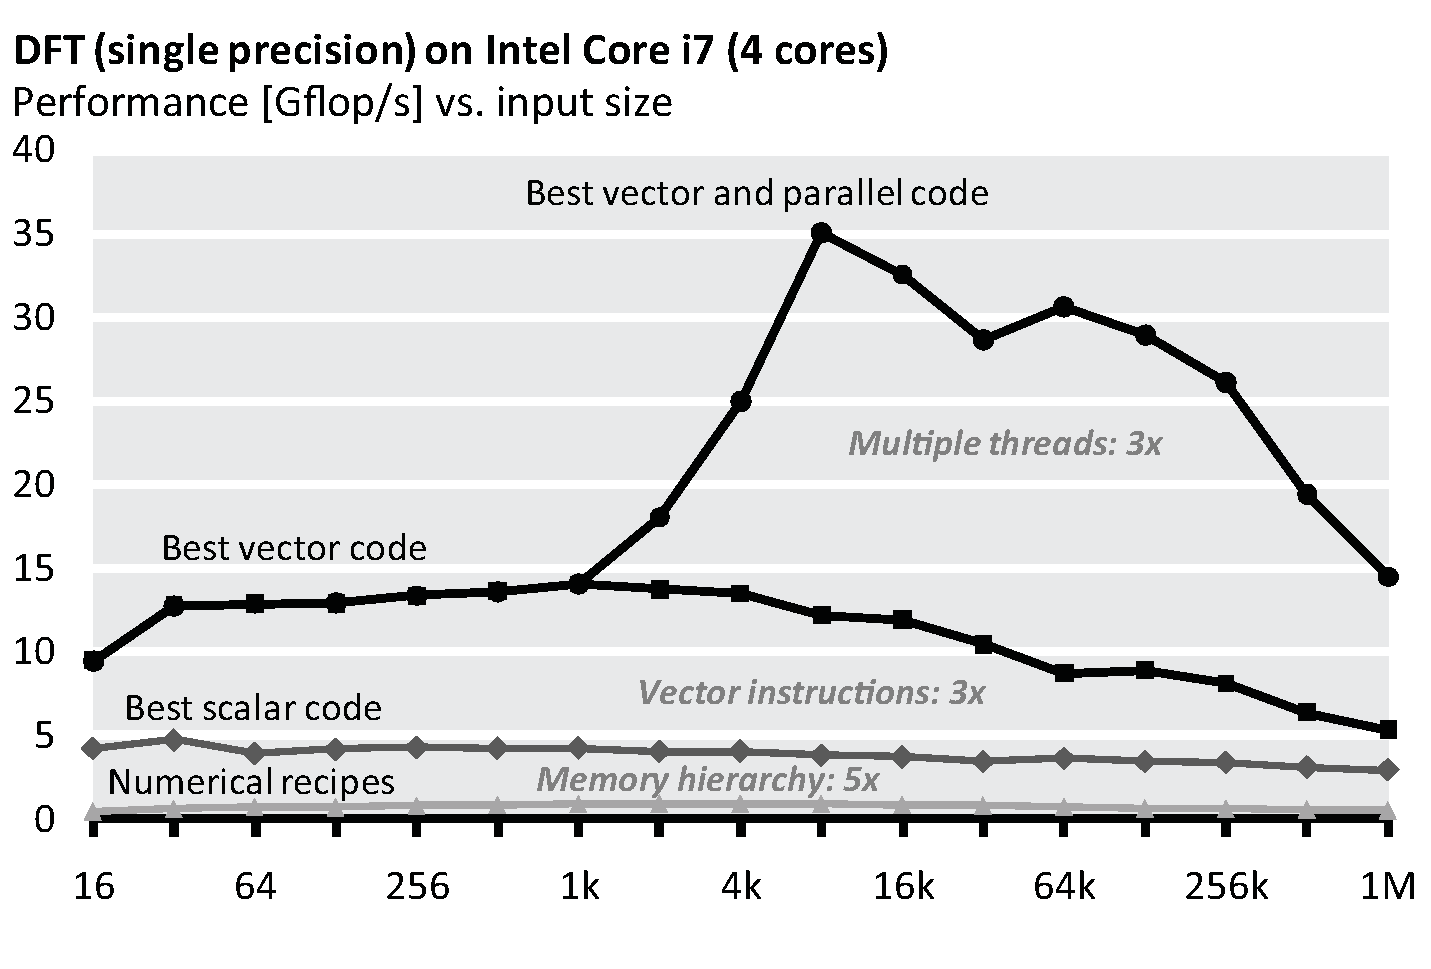
\includegraphics[scale=0.33]{example-plot}
  \caption{Performance of four single precision implementations of the
  discrete Fourier transform. The operations count is roughly the
  same. The labels in this plot are maybe a little bit too small.\label{fftperf}}
\end{figure}

\section{Conclusions}

Here you need to summarize what you did and why this is
important. {\em Do not take the abstract} and put it in the past
tense. Remember, now the reader has (hopefully) read the report, so it
is a very different situation from the abstract. Try to highlight
important results and say the things you really want to get across
such as high-level statements (e.g., we believe that .... is the right
approach to .... Even though we only considered x, the
.... technique should be applicable ....) You can also formulate next
steps if you want. Be brief. After the conclusions there are only the references.

\section{Further comments}

Here we provide some further tips.

\mypar{Further general guidelines}

\begin{itemize}
\item For short papers, to save space, I use paragraph titles instead of
subsections, as shown in the introduction.

\item It is generally a good idea to break sections into such smaller
units for readability and since it helps you to (visually) structure the story.

\item The above section titles should be adapted to more precisely
reflect what you do.

\item Each section should be started with a very
short summary of what the reader can expect in this section. Nothing
more awkward as when the story starts and one does not know what the
direction is or the goal.

\item Make sure you define every acronym you use, no matter how
convinced you are the reader knows it.

\item Always spell-check before you submit (to us in this case).

\item Be picky. When writing a paper you should always strive for very
high quality. Many people may read it and the quality makes a big difference.
In this class, the quality is part of the grade.

\item Books helping you to write better: \cite{Strunk:00}.

\item Conversion to pdf (latex users only): 

dvips -o conference.ps -t letter -Ppdf -G0 conference.dvi

and then

ps2pdf conference.ps
\end{itemize}

\mypar{Graphics} For plots that are not images {\em never} generate the bitmap formats
jpeg, gif, bmp, tif. Use eps, which means encapsulate postscript. It is
scalable since it is a vector graphic description of your graph. E.g.,
from Matlab, you can export to eps.

The format pdf is also fine for plots (you need pdflatex then), but only if the plot was never before in the format 
jpeg, gif, bmp, tif.




\begin{thebibliography}{1}

\bibitem{taflove}
A. Taflove. Computational electrodynamics: The finite-difference time-domain method. 1995.

\bibitem{smith}
G. Smith. Numerical Solution of Partial Differential Equations: Finite Difference Methods. Oxford University Press, 2004.

\bibitem{cong-huang-zou}
J. Cong, M. Huang, and Y. Zou. Accelerating fluid registration algorithm on multi-FPGA platforms. FPL, 2011.

\bibitem{cong-zou}
On the Transformation Optimization for Stencil Computation

\bibitem{su-zhang-mei}
Huayou Su *, Kaifang Zhang and Songzhu Mei. On the Transformation Optimization for Stencil Computation

\bibitem{cruz}
Cruz, R.D.L.; Araya-Polo, M. Algorithm 942: Semi-Stencil. ACM Trans. Math. Softw. 2014, 40, 1–39.

\bibitem{barigou}
Youcef Barigou. Acceleration of real-life stencil codes on GPUs. Hardware Architecture [cs.AR]. 2011.

\bibitem{holewinski-pouchet-sadayappan}
Justin Holewinski, Louis-Noël Pouchet, P. Sadayappan. High-Performance Code Generation for Stencil Computations on GPU Architectures.

\bibitem{techopedia}
Multicore. https://www.techopedia.com/definition/5305/multicore

\bibitem{openmp}
OpenMP. https://www.openmp.org/

\bibitem{loop-interchange}
Loop interchange. https://en.wikipedia.org/wiki/Loop_interchange

\bibitem{optimization-flags}
Options That Control Optimization. https://gcc.gnu.org/onlinedocs/gcc/Optimize-Options.html

\bibitem{parallel-loops}
Parallel Loop Construct. https://www.openmp.org/spec-html/5.0/openmpsu64.html

\bibitem{loop-tiling}
João M.P.Cardoso, José Gabriel F. Coutinho, Pedro C. Diniz. Chapter 5 - Source code transformations and optimizations. Embedded Computing for High Performance

\bibitem{Strunk:00}
W. Strunk~Jr. and E.B. White, \emph{Elements of Style}, 4th ed.\hskip 1em plus
0.5em minus 0.4em\relax Longman, 2000.

\bibitem{IEEEhowto:kopka}
H.~Kopka and P.~W. Daly, \emph{A Guide to \LaTeX}, 3rd~ed.\hskip 1em plus
  0.5em minus 0.4em\relax Harlow, England: Addison-Wesley, 1999.

\end{thebibliography}

\end{document}


